
% NC: Take a look at the JEB instructions for authors. I've done a lot of tweaking for you but this needs to be in a submittable format. So tables and figures at the end etc. I've added line numbers, page numbers etc.

% NC: Might need to have a think about how many tables and figures to include. Fine for thesis but please check JEB guidelines.
	%SF: Manuscript limit is 10 printed pages including figures and tables


%Start: 22/04/14
%Last edited on 28/05

% I sorted out the reference formatting by changing the encoding of my JabRef bibliography file
% Based on my outline for disparity paper_NC_April2014 notes

% Preamble
% NC: I've reordered this a bit (but check it) so that stuff you'll always want is near the top
% and stuff you may need to change depending on the journal is near the bottom

\documentclass[12pt,a4paper]{article}
\usepackage{enumerate} 	% put in numbers or bullet points
\usepackage{setspace}	% line spacing					
\usepackage{authblk}	% For author affiliations
\usepackage{graphicx} 	% For adding pictures

\usepackage[nomarkers]{endfloat} %Figures and tables at the end of the document
\usepackage{pdflscape}	% for landscape pages
\usepackage{mathtools}	% For equations etc.
\usepackage[osf]{mathpazo} % palatino font package

\usepackage{ms}     	% load the manuscript style template

%\usepackage{float}		% Use these options to have figures in specific places in the text
%\floatstyle{plaintop} 	% Force table captions to go above the table

\setcounter{secnumdepth}{0} % removes numbers from section headings
\raggedright 			% justify the text on the left only
\pagenumbering{arabic}	% Page numbers

%\onehalfspacing 		%1.5 line spacing - use the below instead in case you need double spacing for some journals
%\linespread{1.6} 		% this is 1.5 spacing, double line spacing is 1.6 - unrecognised command (maybe due to the setspace package?)
\usepackage[round]{natbib} % author-year citations in round brackets

\title{Cranial morphological disparity within the adaptive radiation of tenrecs (Afrosoricida, Tenrecidae) is no greater than expected by chance} 
% I want to come up with a better title - maybe change it to my talk: Are tenrecs an adaptive radiation?
% NC: Perhaps wait until you have confirmed the results etc.

\author{Sive Finlay$^{1,2,*}$ and Natalie Cooper$^{1,2}$}
\affiliation{\noindent{\footnotesize
$^1$ School of Natural Sciences, Trinity College Dublin, Dublin 2, Ireland.\\ 
$^2$ Trinity Centre for Biodiversity Research, Trinity College Dublin, Dublin 2, Ireland.\\
$^*$sfinlay@tcd.ie; Zoology Building, Trinity College Dublin, Dublin 2, Ireland.\\ Fax: +353 1 6778094; Tel: +353 1 896 2571.\\}}
\date{}	% To give blank date
%Most likely put Steve in here as well
% NC: I have a feeling he may not be interested in being on this one but yes let's ask him

\runninghead{???} %I'll fix this when I have a proper title

\keywords{disparity, morphology, geometric morphometrics, tenrecs, golden moles, adaptive radiation}

% Start of document
\begin{document}

\modulolinenumbers[1] 	% Line numbering on every line

\mstitlepage			% Instead of \maketitle you can use the nice template to get it looking like a manuscript
\parindent=1.5em		% Changes paragraph indenting so it's not so big
\addtolength{\parskip}{.3em} % Changes spacing between sections so it's smaller
%---------------------------------------------------
\begin{abstract}
%I'll do this section last
\end{abstract}

\newpage
%-------------------------------------------------------
\section{Introduction} % NC: This is *far* too long. Best introductions are short and to the point
% NC: What does a reader *really* need to know to understand your paper? Generally aim for 4 or 5 paragraphs. 

% NC: OK I see what you're getting at here. But it's far to long before you get on to what you're actually looking at. How about a severely shortened version, something along the lines of 
%1 - Adaptive radiation, short definition, is an exciting pattern and seen across many taxa (some examples, probably mention Darwin's finches). There has been debate about the exact meaning of the term - some arguing that it should be reserved only for species exhibiting lots of morphological disparity. However, few adaptive radiations have been characterised in this way (if this is true :). 


Adaptive radiations, "evolutionary divergence of members of a single phylogenetic lineage into a variety of different adaptive forms" \citep[Futuyma 1998, cited by][]{Losos2010} have long-attracted the interests and attentions of naturalists. Some of the most famous examples include cichlid fish and Caribbean \textit{Anolis} lizards \citep{Gavrilets2009}. These groups exhibit great variety in both their phenotypic forms and the ecological niches which they occupy. 

Each of these groups are uncontroversially accepted as examples of adaptive radiations. However, there has been considerable debate about how adaptive radiations should be defined (REFS) and how to distinguish an adaptively radiated group from just a clade of apparently diverse species. This is an important distinction because we need a consistent means of identifying an adaptive radiation before we can investigate and understand the selective pressures which cause adaptive radiations to develop in some groups and not others (REFS). 

%-----------------------------
%Maybe put this paragraph in somewhere else but it doesn't fit here
   %I think it's important to make the distinction between taxonomic and phenotypic variety clear. Maybe I could put it into the discussion if it doesn't fit here
%One common issue is the assumption that adaptively radiated (phenotypically and ecologically diverse) groups should also exhibit a high degree of species richness (REFS). This apparent correlation is true for some groups, including the Anole and cichlid examples mentioned above, but taxonomic variety does not necessarily correlate with phenotypic diversity \citep{Ruta2013, Hopkins2013}. Clades that have exceptional phenotypic diversity can still be regarded as adaptive radiations even if they are not taxonomically diverse, the most famous example being Darwin's finches \citep{Gavrilets2009}. 
%--------------
One suggestion which has been proposed is that an adaptively radiated clade should show exceptional (i.e. greater than expected by chance) morphological and ecological diversity \citep{Losos2010a}. In this case, a group of species would be considered exceptionally diverse if they have more phenotypic and ecological diverstiy than their closest relatives and also if they exhibit greater diversity than expected by chance. However, few putative examples of adaptive radiations have been characterised in this way. %I think this is true but I need to double check
Under this definition it is equally important to demonstrate exceptional diversity in both phenotypic variety and the range of ecological niches which the species occupy. However, for the purposes of this paper we will focus on the first criteria; investigating the evidence for morphological variety. 


%2 - Morphological disparity is short definition. It can be measured in many ways including - several *short* methods. 
Phenotypic diversity is commonly measured as morphological disparity; the diversity of organic form \citep{Foote1997,Erwin2007}). There is no single definition of disparity and it can be calculated in many ways including measures of morphospace occupation \citep[e.g.][]{Goswami2011, Brusatte2008} and rate-based approaches that assess the amount of directed change away from an ancestor \citep{OMeara2006, Price2013}. Analyses of disparity apply these alternative approaches depending on whether the study is interested in current patterns of morphological diversity or the rate at which they accumulate through time. 

%I need to finish off the paragraph here depending on whether I end up using one or both approaches 


%3- Here we investigate morphological disparity in tenrecs, to determine whether they represent an adaptive radiation sensu Losos. Tenrecs are - brief description. We use brief methods 

Here we investigate current patterns of morphological disparity in tenrecs (Afrosoricida, Tenrecidae) to determine whether they represent an adaptive radiation sensu \citep{Losos2010a}. The tenrec family is comprised of 34 species, 31 of which are endemic to Madagascar \citep{Olson2013}. From a single common ancestor \citep{Asher2006}, Malagasy tenrecs diversified into a wide variety of descendant species which convergently resemble distantly related insectivore mammals such as shrews (\textit{Microgale} tenrecs), moles (\textit{Oryzorictes} tenrecs) and hedgehogs (\textit{Echinops} and \textit{Setifer} tenrecs) \citep{Eisenberg1969}.

Tenrecs are often cited as an example of an adaptively radiated family which exhibits exceptional morphological diversity \citep{Soarimalala2011, Olson2003, Eisenberg1969}. However, this apparent exceptional diversity is based on subjective comparisons to other groups and it has not been tested quantitatively. If tenrecs are exceptionally morphologically diverse then, following \citep{Losos2010a}, tenrecs should be more morphologically disparate than expected by chance and they should exhibit significantly more phenotypic diversity than their nearest relatives, the golen moles (Afrosoricida, Chrysochloridae). Here we test these predictions using cranial morphology as a proxy for phenotypic diversity.


%4- *Brief$* results and implications. 

Using the most complete morphological data set of tenrecs and golden moles to date we apply geometric morphometric analyses \citep{Rohlf1993, Zelditch2012} to quantify morphological disparity among our species. Our results indicate that, on average, tenrecs are more phenotypically diverse than their closest relatives but their morphological diversity is no greater than that which is expected to evolve by chance.
%NB: the new permutation method shows that only some of these differences are significant 
Therefore, under strict definitions, the designation of tenrecs as an exceptional adaptive radiation may need to be reconsidered. 

These findings highlight the vital importance of testing our common, but often erroneous, expectations about patterns of morphological disparity in groups that exhibit apparent high levels of diversity. 

%I need a better final sentence here
%-------------------------------------------------------------
\section{Materials and Methods}

\subsection{Data collection} % NC: Separate into data collection and analysis sections 
% NC: I'd go for the geometric morphometrics first then mention the supplemental data e.g phylogeny afterwards

\subsubsection{Morphological data collection} % NC: Perhaps more descriptive than geo morph?

% Due to the high number and relatively small sizes of our specimens we chose to use two dimensional morphometrics rather than 3D techniques. NC: Is this needed? Never start a section with an apology!
	%SF Fair point, I was just trying to pre-empt an obvious reviewer criticism but I could stick the justification into the supplemental if necessary
	
One of us (SF) photographed cranial specimens of tenrecs and golden moles at the Natural History Museum London (NHML), the Smithsonian Institute Natural History Museum (SI), the American Museum of Natural History (AMNH), Harvard's Museum of Comparative Zoology (MCZ) and the Field Museum of Natural History, Chicago (FMNH). We photographed the specimens with a Canon EOS 650D camera fitted with an EF 100mm f/2.8 Macro USM lens using a standardised procedure to minimise potential error (see supplementary material for details). 
%NC Might want to use the standard museum abbreviations - BMNH etc.
	%SF I used NHML because I thought the BMNH was the old name?



We collected pictures of the skulls in dorsal, ventral and lateral views (right side of the skull) and of the outer (buccal) side of the right mandibles. A full list of museum accession numbers and access to the images can be found in the supplementary material.


In total we collected pictures from 182 skulls in dorsal view (148 tenrecs and 34 golden moles) and 181 mandibles in lateral view (147 tenrecs and 34 golden moles), representing 31 species of tenrec (out of the total 34 in the family) and 12 species of golden moles (out of a total of 21 in the family \citep{Asher2010}). We used the taxonomy of Wilson and Reeder \citeyearpar{Wilson2005} supplemented with more recent sources \citep{IUCN2012, Olson2013} to identify our specimens. 
% NC: I rearranged to make it shorter, try and do this. Need to be more concise or you'll never get it short enough to submit :)
	%Thanks, I know I'm long-winded!
	

We used a combination of both landmarks (type 2 and type 3, \citep{Zelditch2012}) and semilandmarks to characterise the shapes of our specimens. Our landmarks (points) and semilandmarks (outline curves) used to represent shape variation in the dorsal skulls and mandibles are depicted in Figures \ref{fig:skdors_landmarks} and \ref{fig:mands_landmarks} respectively. Corresponding landmark definitions for each view are in tables \ref{tab:skdors_landmarks} and \ref{tab:mands_landmarks}. We also placed landmarks and semilandmarks on photographs of ventral and lateral skull views, details can be found in the supplementary material. We digitised all landmarks and semilandmarks in tpsDIG, version 2.17 \citep{Rohlf2013}.

%*************************************************
%I've fixed the formatting to put tables and figures at the end
%May need to re-do pictures to grey scale instead of colour
%**************************************
%Skdors landmarks diagram
\begin{figure}
\centering
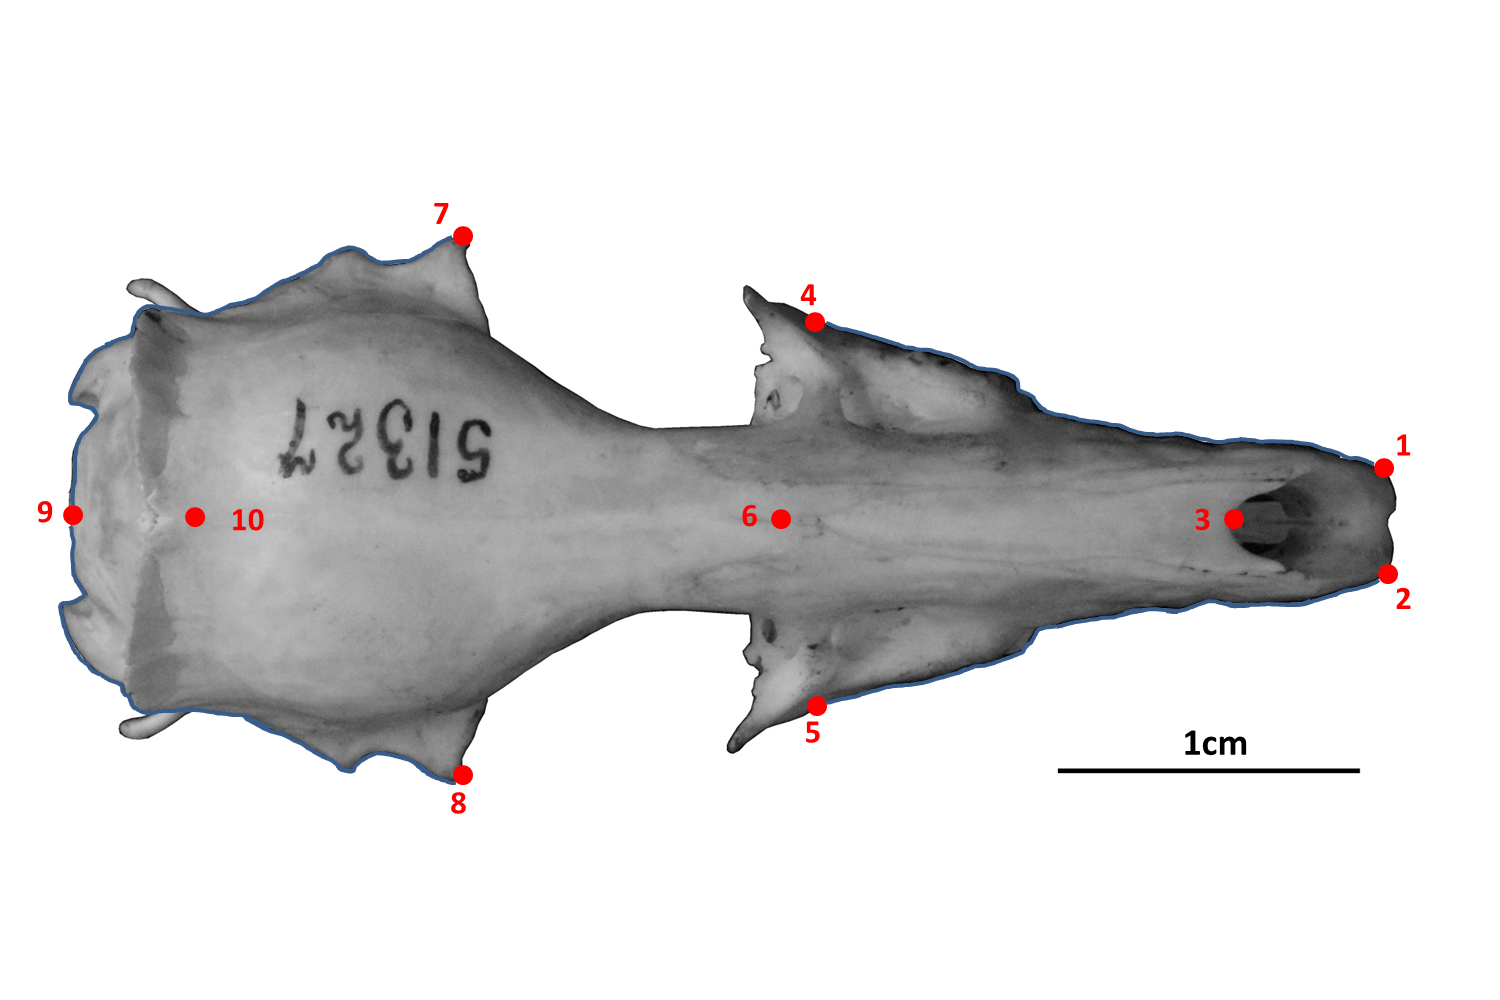
\includegraphics[width=1\linewidth]{figures/AMNH_51327_dorsallandmarksdiagram.png}
\caption{Landmarks (red points) and curves (blue lines) used to capture the morphological shape of skulls in dorsal view. Curves were re-sampled to the same number of evenly-spaced points. See table X for description of curves and landmarks.\textit{Potamogale velox} (Tenrecidae) skull, accession number: AMNH\_51327}
\label{fig:skdors_landmarks}
\end{figure}


%Table for the dorsal skulls landmark descriptions
\begin{table}[H]			
\centering
\caption{Descriptions of the landmarks (points) and curves (semilandmarks) for the skulls in dorsal view (see Figure \ref{fig:skdors_landmarks}).}
%Skdors landmarks

\begin{tabular}[t]{l l}		
\hline
\textbf{Landmark} & \textbf{Description} \\
\hline
%------------------------------------------------------------
1 + 2 & Left (1) and right (2) anterior points of the premaxilla \\
%------------------------------------------------------------
3 & Anterior of the nasal bones in the midline \\
%------------------------------------------------------------
4 + 5 &	Maximum width of the palate (maxillary) on the left (4) and right (5)\\
%------------------------------------------------------------
6 & Midline intersection between nasal and frontal bones \\
%------------------------------------------------------------
7 + 8 & Widest point of the skull on the left (7) and right (8) \\
%------------------------------------------------------------
9 &	Posterior of the skull in the midline \\
	%Panchetti 2008 and Macholan2008 have different definitions for this one so I need to choose one
%------------------------------------------------------------
10 & Posterior intersection between saggital and parietal sutures \\
%--------------------------------------
\hline
\textbf{Curve A} & Outline of the braincase on the left side, between landmarks 9 and 7\\ 
(12 points) & (does not include visible features from the lower (ventral) side of the skull) \\

\textbf{Curve B} & Outline of the palate on the left side, between landamarks 4 and 1 \\
(10 points) & (outline of the rostrum only, not the shape of the teeth)\\

\textbf{Curve C} &	Outline of the braincase on the right side, between landmarks 9 and 8 \\
(12 points) & (does not include visible features from the lower (ventral) side of the skull) \\

\textbf{Curve D} & Outline of the palate on the right side, between landamarks 5 and 2 \\
(10 points) & (outline of the rostrum only, not the shape of the teeth)\\
%------------------------------------------------------------
\hline
\end{tabular} % This is the same table that I used in my methods chapter
\label{tab:skdors_landmarks}  
\end{table}
%------------------------------------------
%Mandibles landmarks diagram
\begin{figure}[H]
\centering
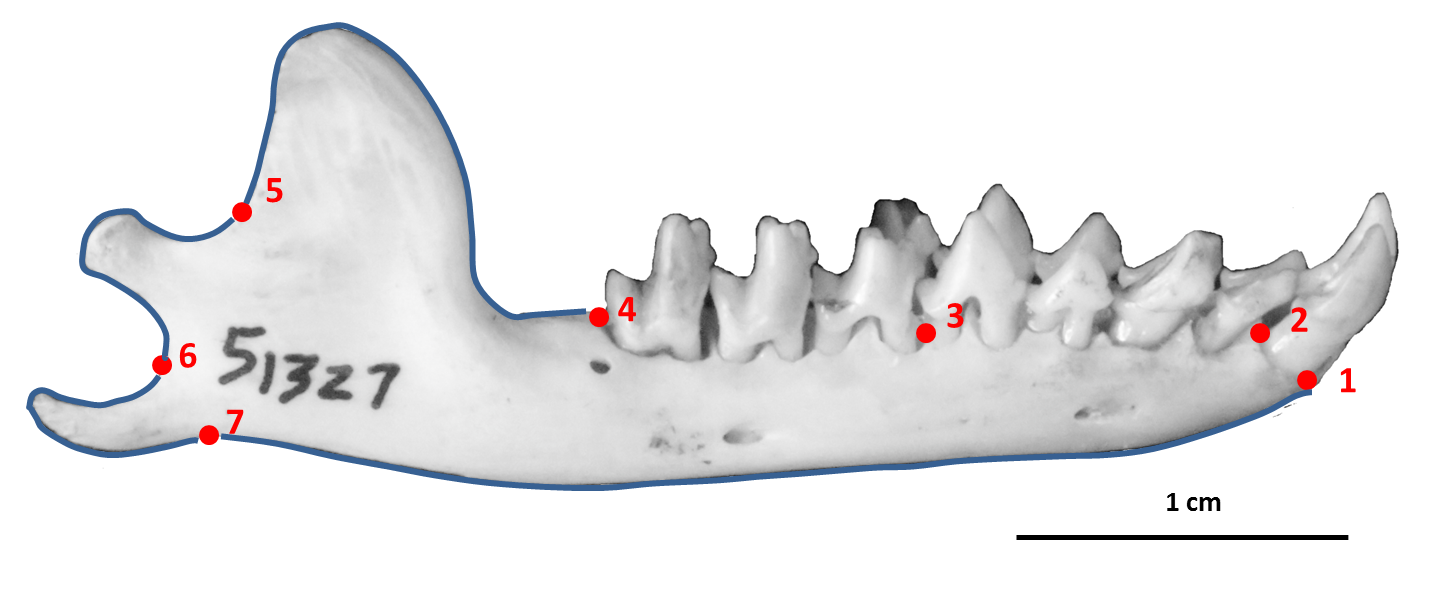
\includegraphics[width=1\linewidth]{figures/AMNH_51327_landmarksdiagram.png}

\caption{Landmarks (red points) and curves (blue lines) used to capture the morphological shape of mandibles. Curves were re-sampled to the same number of evenly-spaced points. See table X for description of curves and landmarks.\textit{Potamogale velox} (Tenrecidae) mandible, accession number: AMNH\_51327}
\label{fig:mands_landmarks}
\end{figure}

%Table for the mandibles' landmark descriptions

\begin{table}[H]			
\centering
\caption{Descriptions of the landmarks (points) and curves (semilandmarks) for the mandibles in lateral (buccal) view (see figure \ref{fig:mands_landmarks})}
%Mandibles landmarks


\begin{tabular}[t]{l l}		
\hline
\textbf{Landmark} & \textbf{Description} \\
\hline
1 & Anterior of the alveolus of the first incisor \\
2 & Posterior of the alveolus of the first incisor \\
3 &	Anterior of the alveolus of the first molar \\
4 & Posterior of the alveolus of the last molar \\
5 & Maximum curvature between the coronoid and condylar processes\\
6 & Maximum curvature between the condylar and angular processes  \\
7 &	Maximum curvature between the angular process and the horizontal ramus \\
%---------------------------------------------------
\hline
Curve A & Condyloid process (between landmarks 4 and 5, 15 points)\\
Curve B & Condylar process (between landmarks 5 and 6, 15 points) \\
Curve C & Angular process (between landmarks 6 and 7, 15 points)  \\
Curve D & Base of the jaw (between landmarks 7 and 1, 12 points)  \\
%---------------------------------------------------
\hline
\end{tabular}


\label{tab:mands_landmarks} %give it a label so I can refer to it in the text
\end{table}
%---------------------------------------------------------- 



We re-sampled the outlines to the minimum number of evenly spaced points required to represent each outline accurately \citep[][details in supplementary material]{MacLeod2013}. We used TPSUtil \citep{Rohlf2012} to create sliders files \citep{Zelditch2012} to define which points were semilandmarks. We conducted all subsequent analyses in R version 3.0.2 \citep[R Development Core][]{Team2013} within the geomorph package \citep{Adams2013}. We used the gpagen function to run a general Procrustes alignment (REFS) of the landmark coordinates while sliding the semilandmarks by minimising procrustes distance rather than bending energy (REFS). We used these Procrustes-aligned coordinates of all species (n=43) to calculate average shape values for each species which we then used for a principal components (PC) analysis (REFS) with the plotTangentSpace function \citep{Adams2013}. 

%-----------------------------------------------
\subsubsection{Phylogeny} 
Instead of basing our analyses on individual trees and assuming that their topologies were known without error \citep[e.g.][]{Ruta2013, Foth2012, Brusatte2008, Harmon2003} we used a distribution of 101 pruned phylogenies derived from the randomly resolved mammalian supertrees in \citep{Kuhn2011}. 
	% I used 101 because that was the number in the smaller Fritz file - I could change it to 100 instead if 101 sounds odd?

Eight species (six \textit{Microgale} tenrecs and two golden moles) in our morphological data were not in the phylogenies. Phylogenetic relationships among the \textit{Microgale} have not been resolved more recently than the \citep{Kuhn2011} analysis, therefore we added the additional \textit{Microgale} species at random to the \textit{Microgale} genus within each phylogeny \citep{Revell2012}. We could not use the same approach to add the two missing golden mole species because they were the only representatives of their respective genera within our data. Therefore we randomly added these species to the common ancestral node (using the findMRCA function in phytools \citep{Revell2012}) of all golden moles within each phylogeny. Adding these extra species to the phylogenies created polytomies which we resolved arbitrarily using zero-length branches \citep{Paradis2004}. We calculated pairwise phylogenetic distances among species using the cophenetic function \citep[R Development Core][]{Team2013}. 
% NC: I feel like some of this belongs in the analysis section...
	%SF It could do but I'm not sure where to put it without making a separate analyses section for the phylogenies and I don't think that makes sense.  
	
%-------------------------------------------------------	
\subsection{Analyses}
\subsubsection{Disparity calculations} 

We calculated morphological disparity separately for golden moles and tenrecs in each of the morphological datasets. We used the PC axes which accounted for 95\% of the cumulative variation to calculate four disparity metrics; the sum and product of the range and variance of morphospace occupied by each family \citep{Brusatte2008, Foth2012, Ruta2013}. We also calculated morphological disparity directly from the Procrustes-superimposed shape data \citep[ZelditchMD,][]{Zelditch2012}. 
Disparity is expected to be higher in larger groups (REFS). Therefore we repeated our disparity comparisons between the two families using rarefaction (see supplementary material) to confirm that observed differences in disparity between the two groups were not artefacts of differences in sample size.
%Remember to change this part when I do the new analysis using Steve Wang's code
 %- Group comparisons based on permutation tests so there's no need for rarefaction analyses

To test whether tenrecs are more morphologically disparate than expected by chance, we simulated shape evolution  \citep{Harmon2008} of the species-average, Procrustes-superimposed shape coordinates of each tenrec species across our distribution of phylogenies. We took "chance" to mean the expected shape evolution under a Brownian Motion (BM) model and we repeated 1000 simulations on of shape evolution in BM on each of 101 phylogenies pruned to include tenrec species only. We ran a principal components analysis on each of the simulations and used the PC axes which accounted for 95\% of the cumulative variation to calculate disparity metrics.

We compared the observed disparity measure to the corresponding distribution of values and used a two-tailed test to determine whether the observed (true) disparity measures were more or less than that which is expected to evolve under BM.

The majority of tenrecs (19 out of 31 in our data) are members of the \textit{Microgale} (shrew-like) genus which is notable for its relatively low phenotypic diversity \citep{ Soarimalala2011, Jenkins2003} and may mask signals of high disparity among other tenrecs. To test this we repeated our simulations of shape evolution excluding \textit{Microgale} species. This reduced our data set for tenrecs from 31 to 12 species. 

To test whether tenrecs have significantly different morphologies than golden moles, we used a non parametric MANOVA \citep{Anderson2001} to compare morphospace occupation between the two groups (REFS?). %Doesn't test for differences in disparity, just the areas of morphospace which they occupy 
%Permutation tests, not overlap of confidence intervals to see if there's a significant difference in disparity between the two groups

%-----------------------------------------------------------

\section{Results}

\subsection{Morphological disparity in tenrecs} 


%***************************************
% NC: Rethink subheadings - best idea is if they match the methods, if not then maybe no subheadings are required.
%*****************************************

We compared observed disparity to the distributions of expected disparity calculated from BM simulations of shape data (1,000 simulations on each of 101 phylogenies). We present the results from comparing our observed and simulated measures of sum of variance (figures \ref{fig:skdors_sumvar} and \ref{fig:mands_sumvar}) because all disparity metrics yielded the same patterns: tenrecs have significantly lower disparity than expected under BM.  Full results from all disparity metrics and including the ventral and lateral skull views can be found in the supplementary.

%I moved the summary tables to the supplementary and put the figures in instead
%*****************************************
%Sum of variance diagrams -overall dissimilarity, less affected by sample size Wills 1994

%Figures of simulated compared to observed disparity measures

\begin{figure}
\centering
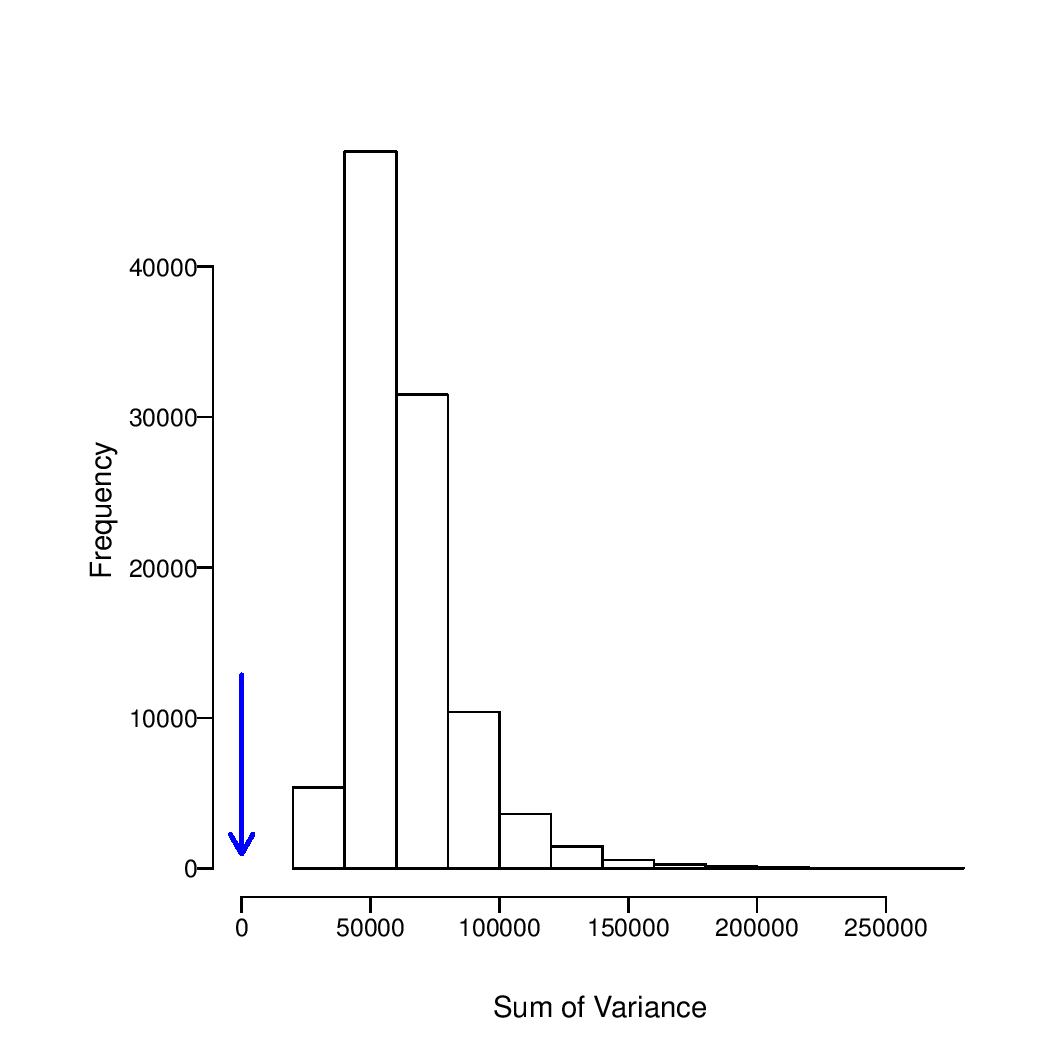
\includegraphics[width=1\linewidth]{figures/skdors_trc+gmole_tenrec_sumvariance.jpg}

\caption{Comparison of the observed and expected disparity in the dorsal skulls. Disparity is measured as sum of variance, blue arrow points to the observed value of disparity (0.0017)}
\label{fig:skdors_sumvar}
\end{figure}

\begin{figure}
\centering
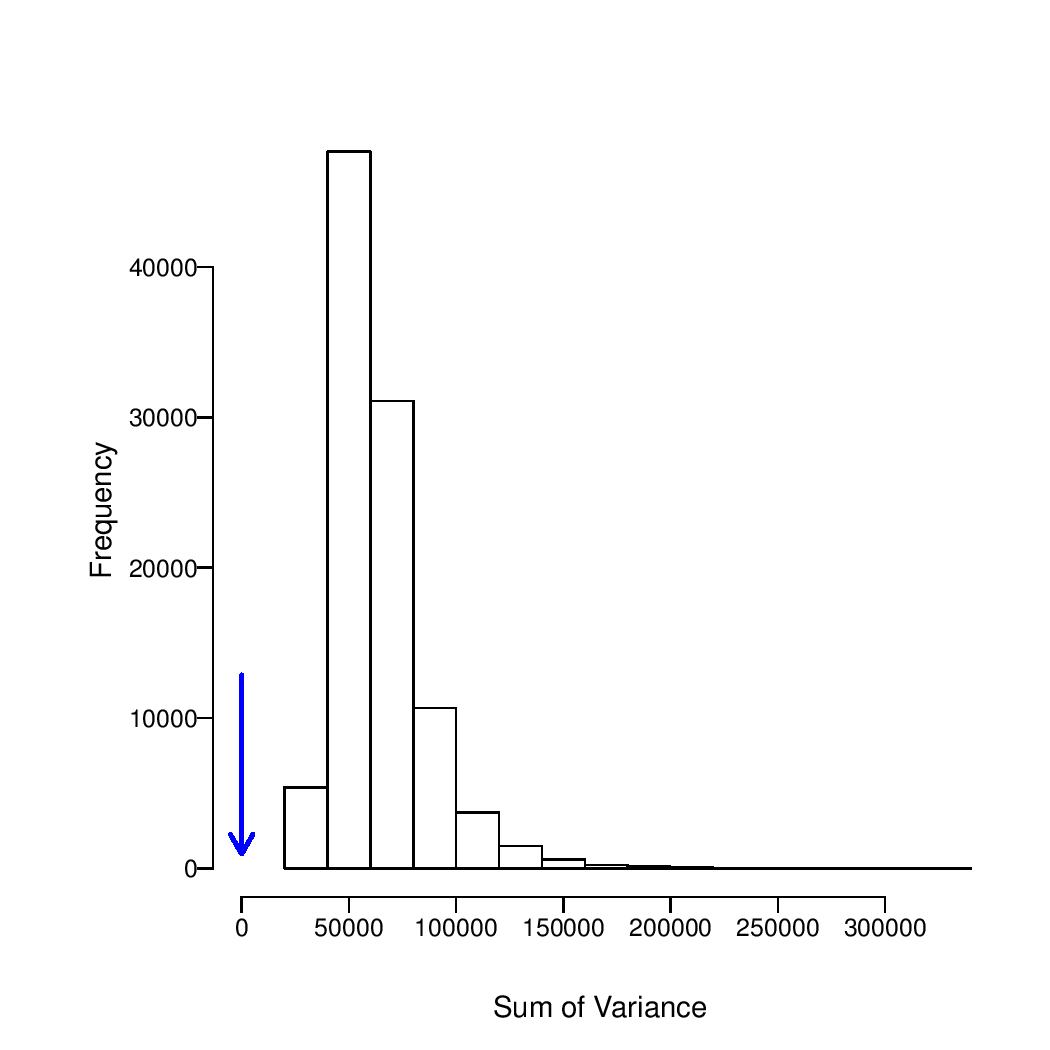
\includegraphics[width=1\linewidth]{figures/mands_trc+gmole_tenrec_sumvariance.jpg}

\caption{Comparison of the observed and expected disparity in the mandibles. Disparity is measured as sum of variance, blue arrow points to the observed value of disparity (0.0031)}
\label{fig:mands_sumvar}
\end{figure}



%********************************************************

Removing the phenotypically similar \textit{Microgale} tenrecs did not qualitatively affect our results; the non-\textit{Microgale} tenrecs still show significantly lower phenotypic disparity than expected by chance (simulation results in the supplementary material). 


%******************************************************

\subsection{Morphological disparity in tenrec and golden moles} 

Figures  \ref{fig:skdorsPCA} and \ref{fig:mandsPCA} depict the morphospace plots derived from our principal components analyses of average Procrustes-superimposed shape coordinates for each species in our skull and mandible data respectively. We used the principal components axes which accounted for 95\% of the cumulative variation (n = 6 axes for the dorsal skulls analysis and n = 11 axes for the mandibles) to calculate the disparity of each family. 

In the dorsal skulls analysis, tenrecs and golden moles occupy significantly different areas of morphospace (npMANOVA, F = 59.34, R$^2 $ = 0.59, p = 0.001) indicating that the two families have signficantly different skull morphologies. 
%These are the npMANOVA results based on the PC axes rather than the distance matrix
For each of the calculated metrics, tenrecs have higher disparity than golden moles but these differences were not significant for the variance-based calculations.  



%Not much point in mentioning the non-Microgale tenrecs here because you would expect them to have higher disparity anyway
%Non-\textit{Microgale} tenrecs also have higher disparity than golden moles and we found the same results in our analyses of ventral and lateral skull shapes (see supplementary material).

Tenrecs and golden moles also have significantly different mandible shapes (npMANOVA F = 59.34, R$^2$ = 0.59, p =	0.001). However, unexpectedly, golden moles appear to have higher disparity than tenrecs in the shape of their mandibles (significant differences when disparity is calculated as product of variance, sum of ranges and ZelditchMD).   

We tested whether these results may be artefacts of relatively low phenotypic diversity within \textit{Microgale} tenrecs. However, although golden moles and non-\text{Microgale} tenrecs occupy significantly different areas of morphospace (npMANOVA F = 31.6, R$^2$ = 0.59, p =	0.001), there is no significant difference between the two groups for any metrics of disparity. %based on the permutation tests



%************************************
%PCA figures
%I want to make these figures nicer

	% I could add the warp grids but they look messy and would be very small
	% Change points to be different shapes rather than colours?
	% Goswami2011 has more interesting graphs but probably overly complicated - points are different silhouettes of animals, they show the extremes with wireframe models which are neater than warp grids
	% NB: there are charges for colour printing

% NC: Simple and clear is best.
	
\begin{figure}[H]
\centering
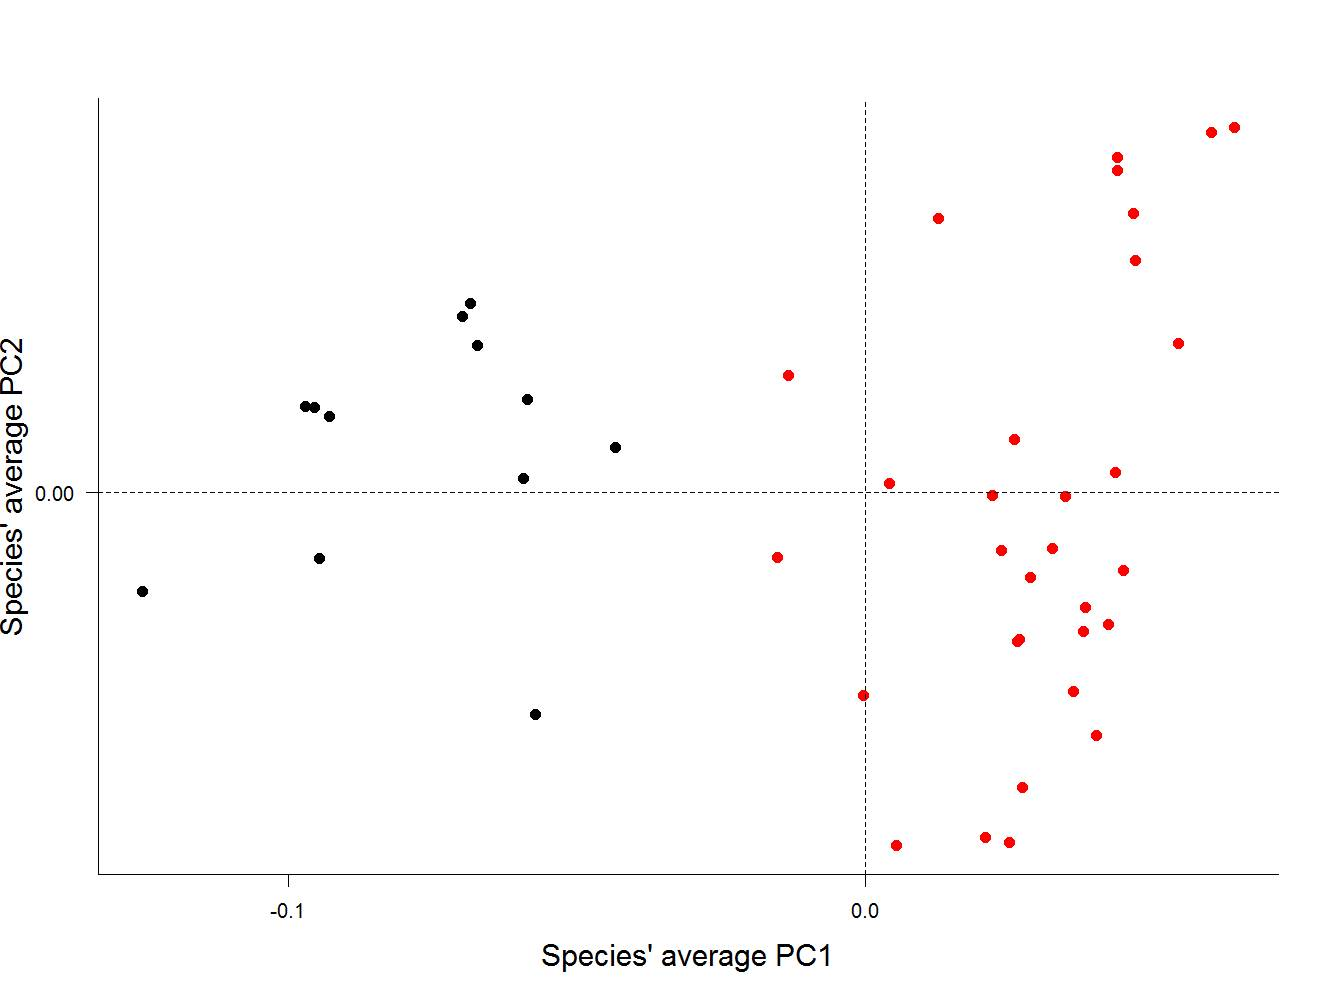
\includegraphics[width=1\linewidth]{figures/SkDors_Tenrecs+Gmoles_PC1PC2_01_05.jpg}
\caption{Principal components plot of the dorsal skulls' morphospace occupied by tenrecs (red, n=31) and golden moles (black, n=12). Axes are PC1 and PC2 of the average scores from a PCA analysis of mean Procrustes shape coordinates for each species. }
\label{fig:skdorsPCA}
\end{figure}


\begin{figure}[H]
\centering
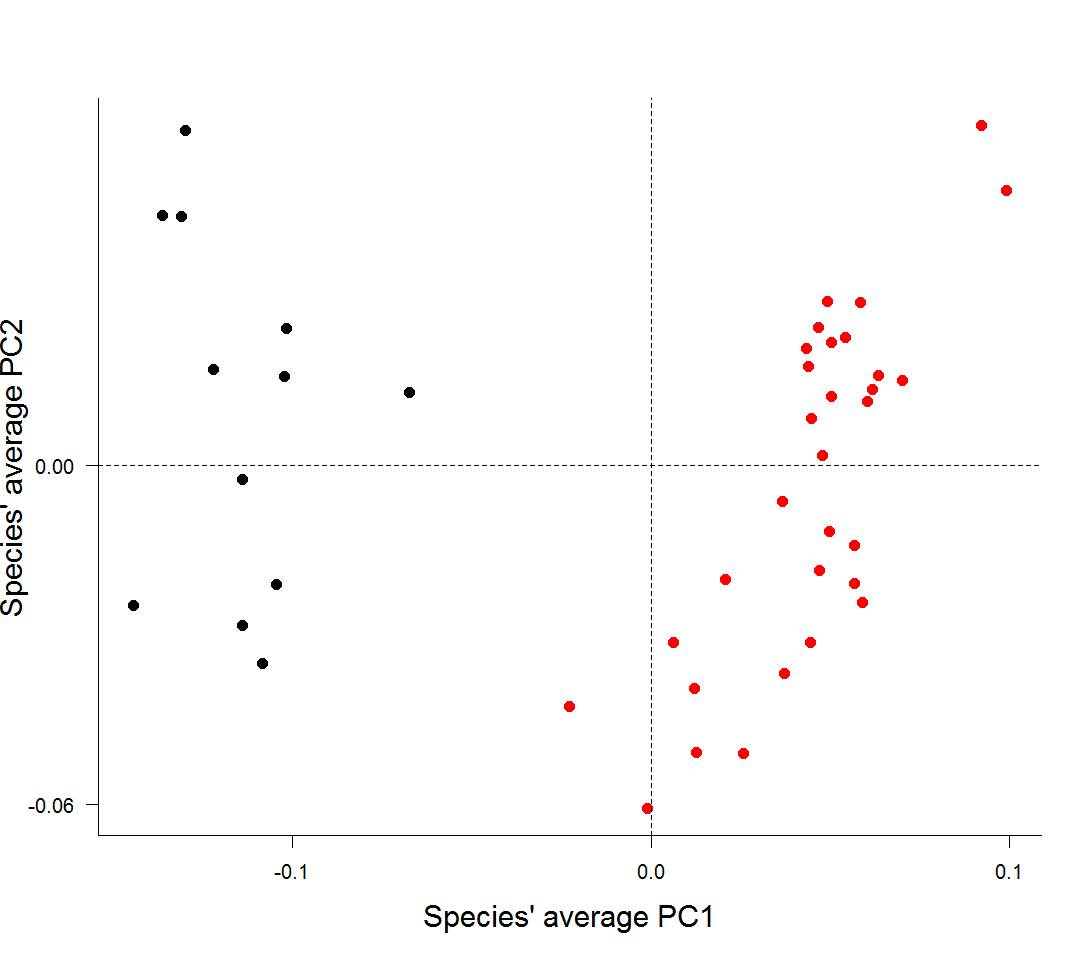
\includegraphics[width=1\linewidth]{figures/Mands_Tenrecs+Gmoles_PC1PC2_01_05_14.jpg}
\caption{Principal components plot of the mandibles' morphospace occupied by tenrecs (red, n=31) and golden moles(black, n=12). Axes are PC1 and PC2 of the average scores from a PCA analysis of mean Procrustes shape coordinates for each species. }
\label{fig:mandsPCA}

\end{figure}
%**********************************************


\section{Discussion} % NC: I know this is rough and hard to do before the final results are in, so I haven't done too much to it. It looks a bit long already though. Same kind of rules apply as in the introduction. 
%Discussion is mainly meant to set your results in the context of other work. You don't need to include every little possible problem in the caveats.


%1 - summary of results
Our findings provide new insights into phenotypic diversity within the tenrec family. Contrary to previous suggestions \citep[e.g.][]{Eisenberg1969, Olson2013}, tenrecs do not appear to be exceptional in their morphological diversity. They do seem to be more morphologically disparate than their closest relatives but only in skull morphology; the opposite is true when we look at mandible morphology (figure \ref{fig:mandsPCA}). Our results illustrate the vital importance of applying quantitative methods to test assumptions about morphological diversity. 

%2 - interpret results with reference to other work

Tenrecs are evidently a diverse group, both phenotypically and ecologically. Body sizes of extant tenrecs span three orders of magnitude (2.5 to \textgreater 2,000g) which is a greater range than all other Families, and most Orders, of living mammals \citep{Olson2003}. Within this vast size range there is striking morphological diversity, from the spiny \textit{Echinops, Setifer} and striking \textit{Hemicentetes} to the shrew-like  \textit{Microgale}. Furthermore, tenrecs inhabit a variety of ecological niches and habitats including terrestrial, arboreal, semi-aquatic and semi-fossorial forms (REFS).

However, our results cast doubt over whether the evident diversity within the tenrec family should be considered to be an adaptive radiation. Phenotypic and ecological divergences within a clade are not surprising; most clades have at least small levels of disparity so, when it comes to identifying adaptive radiations, it's important to identify clades which are exceptional in their diversity \citep{Losos2010a}. Here we have presented the first quantitative investigation of morphological disparity in tenrecs and our results suggest that perhaps phenotypic variation in tenrecs is not the product of an adaptive radiation in the strict sense of its definition.

Although tenrecs are not more morphologically diverse than expected by chance, they do show greater cranial disparity than their nearest relatives. The discrepancies between our analyses of cranial and mandible disparity could reflect derive from factors associated with the modularity of morphological evolution.

There is strong evidence that morphological variation in skulls and mandibles is derived from differential evolution of integrated developmental modules \citep[reviewed by][]{Klingenberg2013a}.
For example, there seems to be two primary modules in the mouse mandible; an alveolar part which holds the teeth and the ascending ramus for muscle attachment and which articulates with the skull \citep{Klingenberg2008a}. Geometric shape covariation is stronger within rather than between these modules. 

Our landmarks and curves for the mandibles (figure \ref{fig:mands_landmarks}, table \ref{tab:mands_landmarks}) include aspects of variation in the dentition but they focus particular attention on the ascending ramus (condyloid, condylar and angular processes). Therefore the higher morphological disparity in golden mole mandibles most likely reflects greater variation in the shape of the muscle attachment areas of the mandible. In contrast it proved impossible to position reliable landmarks on the corresponding articulation areas of the skull in lateral view (see supplementary).

If variation in muscle attachment/articulation sites is driving morphological disparity in mandibles, it is not clear why golden moles should have more disparate articular rami than tenrecs. 

% SF Grasping at straws here, I still don't have a reason why golden moles should have more variable muscle attachment sites than tenrecs
 
% NC: Really need to come up with some vague biological explanation before saying it's all errors in my data collection

% SF The results could still change when I fix the code

%3 - Caveats
While our findings cast doubt on the designation of tenrecs as an adaptive radiation sensu \citep{Losos2010a}, there are certain caveats to consider which could modify the interpretation of our results.

%No test of adaptive significance
Phenoypic variation can evolve for reasons other than adaptive radiation. Therefore, to describe phenotypic divergence as the product of an adaptive radiations requires exceptional morphological diversity in traits which have specific and proven adaptive significance \citep{Losos2010a}. The evolution of cranial shape (both upper skull and mandible), particularly dental morphology, has obvious correlations with dietary specialisations (REFS) and occupation of specific ecological niches (REFS). 

%maybe references for specific head shape in digging mammals? 

Considering the wide ecological diversity of our study species; the fossorial golden moles and semi-fossorial, arboreal, terrestrial and semi-aquatic tenrecs (REFS) it is reasonable to expect that variation in cranial shape should be an adaptive characterstic which allows the animals to survive in their divergent niches. Therefore quantifying the diversity of cranial morphology is a reasonable method of assessing the significance of morphological variety within the context of identifying an adaptive radiation.
%I know this is weak; maybe I should just say that we didn't measure whether skull shape is adaptive but equally neither did any other study?

%Skulls don't measure all diversity
Cranial shape similarities are commonly used to delineate species boundaries (REFS) or for cross-taxonomic comparative studies of phenotypic (dis)similarities (REFS). However, disparity studies are inevitably constrained to be measures of diversity within specific traits rather than overall morphology \citep{Roy1997}. Therefore it is possible that other morphological proxies of phenotype; analyses of linear measurements and/or discrete characters of either cranial or post-cranial morphologies could yield different results. 

However, the results of \citep{Foth2012} are encouraging. In an analysis of morphological disparity in pterosaurs, they found that disparity calculations based on geometric morphometric characterisation of skull shape yielded broadly similar results compared to analyses of whole-skeleton discrete characters and limb proportion data sets. Therefore the disparity patterns we find here based on geometric morphometric analyses of cranial shape most likely represent approximations of disparity which are accurate for morphological diversity in the clades. 

% NC: Is this relevant to our results? Did we really do enough to say we looked into discrepancies? Maybe we did, I'm just trying to get you to be critical of what you include.

%***************************************************************
	% maybe I make the point too strong but I think it's important to mention it somewhere, otherwise it would be an easy criticism from a reviewer to say that we're basing a broad test of adaptive radiation on very limited assumptions of disparity from just skulls
%******************************************************


%Extinction
% NC: This may not be all that important here
	% SF; I've taken it out for now
%We have only measured disparity in extant tenrecs as there is a paucity of fossil forms (REFS). Phenotypic diversity of extant members of a clade are often incomplete representations of the total morphological diversity of that clade over evolutionary time (REFS). Therefore it is possible that current diversity trends in extant taxa are not accurate representations of overall disparity within the entire tenrec clade. 


%4 - Implications
% I still need to do the final paragraph





%Of course cranial diversity is only one aspect of morphological dispariy and more analyses are needed but this is still interesting/relevant because it's the first to test whether phenotypic diversity in tenrecs is more than skin deep/greater than expected by chance

\section*{Acknowledgements}

We thank Dr. Fran\c{c}ois Gould, Thomas Guillerme and the members of NERD club for insightful discussions and the musuem staff and curators for their support and access to collections. Funding was provided by an Irish Research Council EMBARK Initiative Postgraduate Scholarship (SF) and the European Commission CORDIS Seventh Framework Programme (FP7) Marie Curie CIG grant. Proposal number: 321696 (NC, SF)

\bibliographystyle{jeb}
\bibliography{Refs_01_05_14_edited}
% I downloaded the jeb.bst file from http://schneider.ncifcrf.gov/latex.html but there isn't an associated style file

% NC: You can make one via the command line as I showed you in one of my LaTeX lessons.

	%**********************
	%SF: I need to do this so that the references have the abbreviated journal titles, don't include the doi and don't include the total number of pages in books
	%*******************************************

%\bibliography{Refs_01_05_14_edited} %this contains all of the references in my EndNote library on the 01/05/14
%Remeber to edit references within JabRef: put in the LaTex code for special symbols and I also had to go through each title and put \textit{} for italics species names and {} around capital letters because otherwise that formatting doesn't come out in the final document, I also changed the encoding to UTF-8 because that was the only way to get the references to come out as surname before the first name


\end{document}